\chapter{Zbieranie i przetwarzanie danych z czujników}

\section*{Raspberry Pi}

Wszystkie zestawy zbudowano w oparciu o Raspberry Pi 3 v1.2. Zdecydowano się na to rozwiązanie, ponieważ bazuje on na dystrybucji Linuxa, posiada opowiednie interfejsy i złącza a także zintegrowany moduł WiFi. Minusem w stosunku do konkurencyjnego Arduino jest brak wejść analogowych. Problem rozwiązano dodając zewnętrzny przetwornik A/C.
\paragraph{Specyfikacja Raspberry Pi 3:}
\begin{itemize} 
\item Procesor 1.2 GHz
\item Liczba rdzeni 4. Quad Core
\item Pamięć RAM 1 GB
\item Pamięć Karta microSD
\item 40 GPIO
\end{itemize}
\begin{figure}[h]
	\centering
	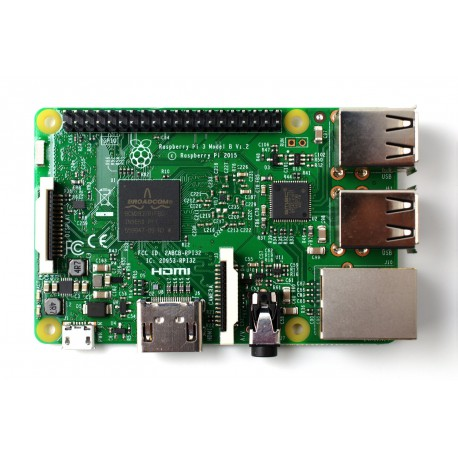
\includegraphics[width=6cm]{raspberry.jpg}
	\caption{Raspberry Pi 3}
\end{figure}
Aby prawidłowo zainstalować oprogramowanie The Guard na dowolnym urządzeniu Raspberry Pi 3 należy wykonać poniższe czynności w terminalu:
\begin{enumerate} 
\item sudo apt-get install libx264-dev
\item cd /usr/src
\item git clone git://source.ffmpeg.org/ffmpeg.git
\item sudo ./configure --arch=armel --target-os=linux --enable-gpl --enable-libx264 --enable-nonfree
\item sudo make
\item sudo install
\item sudo nano /boot/config.txt
\item dopisać w pliku Dtoverlay=w1-gpio i Gpiopin=4
\item pip intall wiringpi
\item sudo pip install spidev
\item pip install pyrebase
\end{enumerate}
Następnym krokiem jest włączenie odpowiednich interfejsów w panelu konfiguracyjnym. Należy zmienić ustawienia zgodnie z poniższym schematem:
\begin{figure}[h]
	\centering
	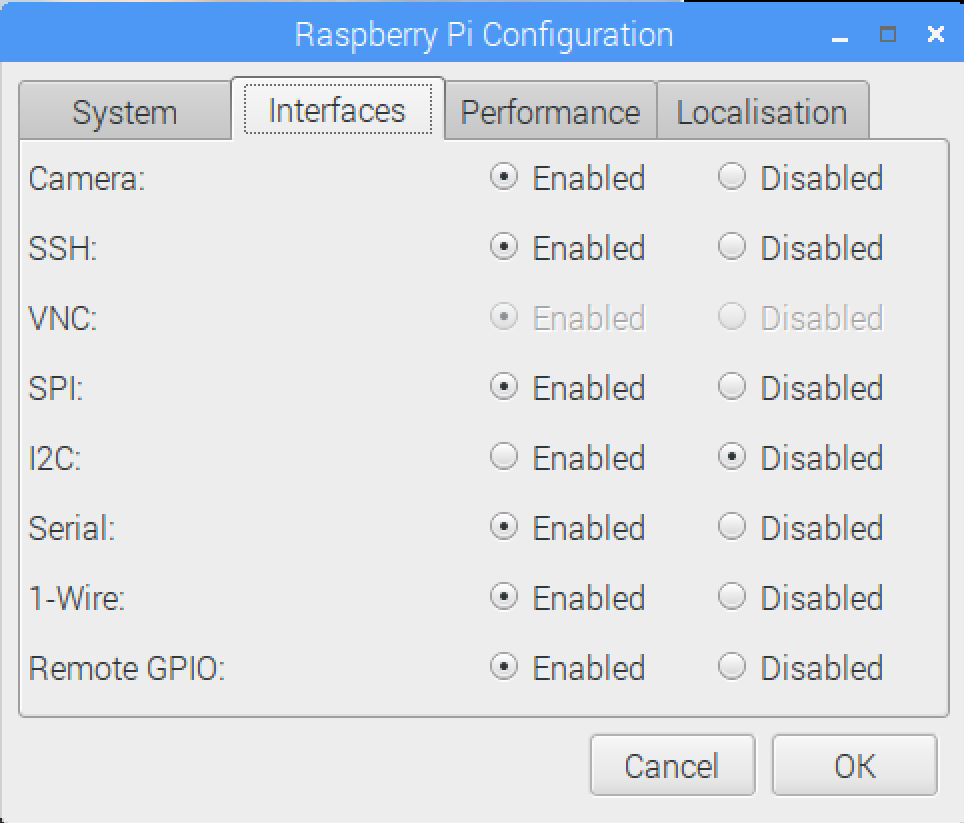
\includegraphics[width=6cm]{RSettings}
	\caption{Ustawienia}
\end{figure}
W kodzie użyto biblioteki wiringpi do odczytu danych z układów cyfrowych. Należy podkreślić, że numeracja fizycznych pinów i numeracja pinów w bibliotece wiringPi jest różna i nie zawiera wszystkich dostępnych pinów na urządzeniu. Przykładowo odczyt pinu 1 w wiringPi jest równoznaczny z odczytem stanu na pinie 12 (GPIO18) na fizycznym urządzeniu.
\begin{figure}[h]
  \centering
  \begin{minipage}[b]{0.4\textwidth}
    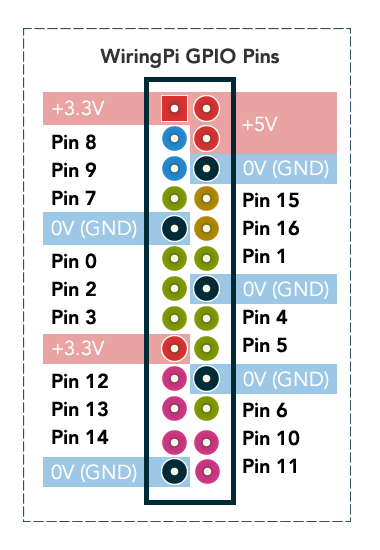
\includegraphics[width=\textwidth]{wiringpi.png}
    \caption{WiringPi}
  \end{minipage}
  \hfill
  \begin{minipage}[b]{0.4\textwidth}
    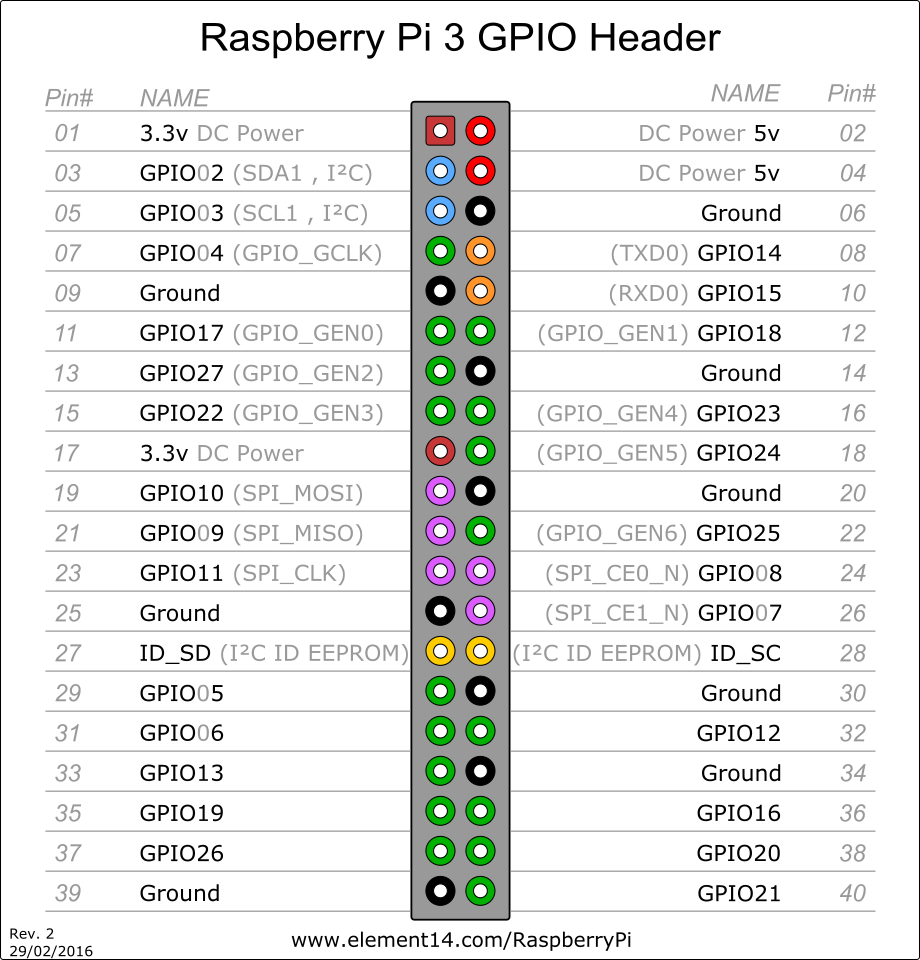
\includegraphics[width=\textwidth]{gpio.png}
    \caption{GPIO}
  \end{minipage}
\end{figure}
Oprogramowanie zainstalowane na Raspberry Pi odpowiedzialne jest za ciągłe monitorowanie stanów i danych z czujników pomiarowych. Po podłączeniu układu do zasilania program jest uruchamiany automatycznie. Pierwszą czynnością jaką wykonuje Raspberry jest wysłanie swojego numeru seryjnego do bazy danych Firebase. Cały proces jest w pełni zautomatyzowany. Dzięki temu użytkownicy od razu mogą dodać urządzenie i monitorować dane z czujników na aplikacjach klienckich. Dodawanie urządzenia następuje poprzez wprowadzenie w aplikacji numeru seryjnego urządzenia.

\section*{Czujniki}
Każdy zestaw składa się z 5 czujników analogowo cyfrowych,  jednej kamery i jednego przetwornika AC. 
\paragraph{a) Specyfikacja MQ-9 - czujnik tlenku węgla:}
\begin{itemize} 
\item Zasilanie: 5 V
\item Pobór prądu: 150 mA
\item Temperatura pracy: od -10 do 50 \textdegree{}C
\item Wyjścia: analogowe oraz cyfrowe
\end{itemize}

\paragraph{b) Specyfikacja MQ-2 - czujnik LPG i dymu:}
\begin{itemize} 
\item Zasilanie: 5 V
\item Pobór prądu: 150 mA
\item Temperatura pracy: od -10 do 50 \textdegree{}C
\item Wyjścia: analogowe oraz cyfrowe
\end{itemize}

\paragraph{c) Specyfikacja czujnika wykrywania płomieni:}
\begin{itemize} 
\item Zasilanie: 3.3 V
\item Zakres wykrywanej fali: 760 do 1100nm
\item Kąt detekcji: od 0 do 60 stopni
\item Temperatura pracy: od -25 do 85 \textdegree{}C
\end{itemize}

\paragraph{d) Specyfikacja DS18B20 - czujnik temperatury:}
\begin{itemize} 
\item Zasilanie: 3.3 V
\item Zakres pomiarowy: od -55 do 125 \textdegree{}C
\end{itemize}

\paragraph{e) Kamera:}
\begin{itemize} 
\item Wykorzystano moduł kamery Raspberry Pi element14
\item Kamera 5MP - wspierająca nagrywanie 30 klatek na sekundę w rozdzielczości Full HD
\end{itemize}

\paragraph{f) Specyfikacja MCP3008 - przetwornik A/C:}
\begin{itemize} 
\item Zasilanie: od 2.7V do 5.5V
\item Pobór prądu: 0.5 mA
\item Interfejs komunikacyjny: SPI
\item Liczba kanałów: 8
\item Rozdzielczość: 10bit
\item Czas konwersji: 10us
\end{itemize}

\begin{figure}[h]
	\centering
	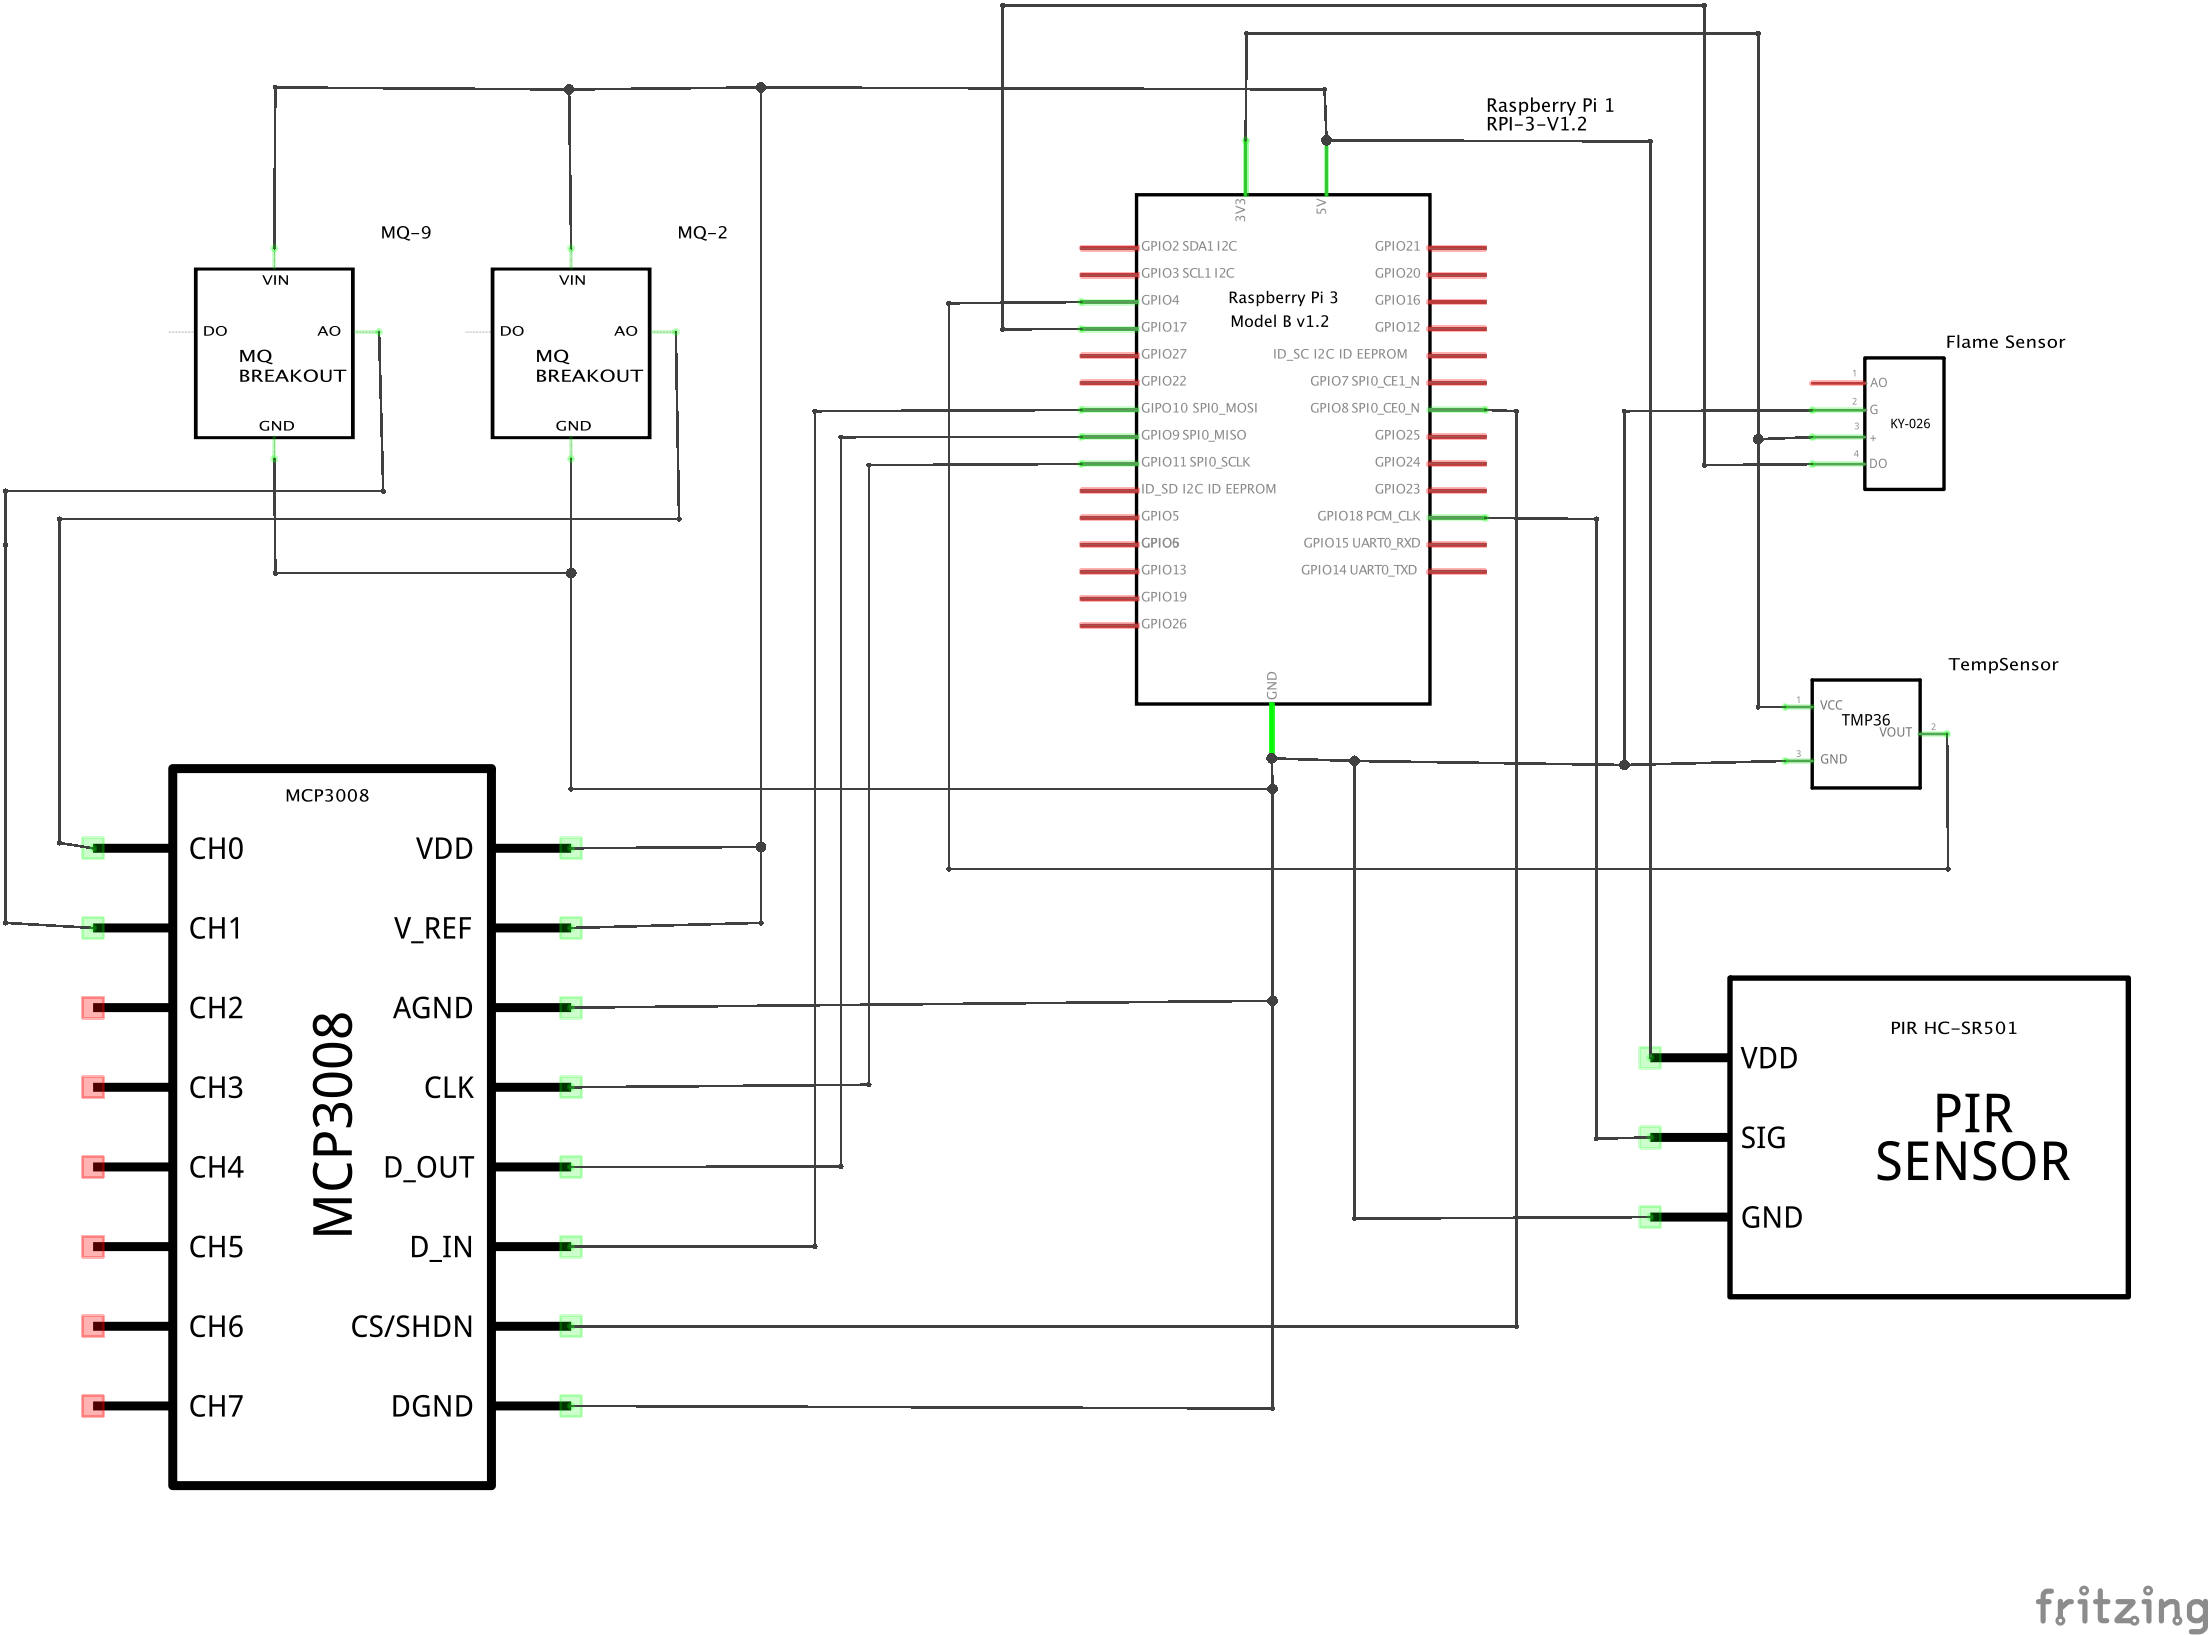
\includegraphics[width=15cm]{GuardSchem}
	\caption{Schemat układu The Guard}
\end{figure}

Niestety żaden model Raspberry nie posiada wbudowanego przetwornika analogowo cyfrowego dlatego konieczne było użycie układu zewnętrzenego. Wybraliśmy przetwornik MCP3008 ze względu na jego nisko koszt i interfejs SPI, który jest wspierany przez Raspberry Pi.
MCP3008 to 10-bitowy przetwornik analogowy cyfrowy. Zasilany jest napięciem 5V, napięcie VRef = 5V.  Skoro jest to przetwornik 10-bitowy jest w stanie wykryć 1024 stany. Wykrywana przez niego minimalna różnica napięć na wejściu wynosi 
\begin{equation}
1 * 5V / 1024 = 4.88mV
\end{equation}
Posiada 8 kanałów jednak w projekcie wykorzystano tylko 2 – do podłączenia czujników MQ-9 i MQ-2.

\paragraph{Interfejs SPI:}
\begin{figure}[h]
	\centering
	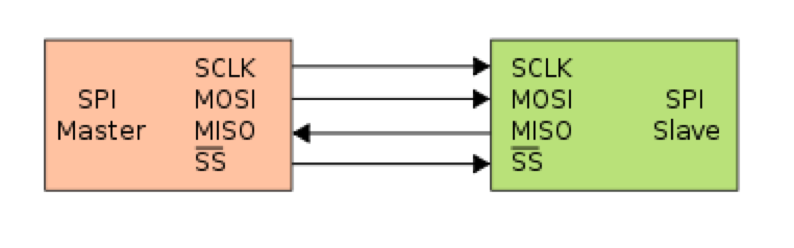
\includegraphics[width=6cm]{SPI.png}
	\caption{Interfejs SPI}
\end{figure}
SPI jest to interfejs synchroniczny. Może być do niego podłączone wiele urządzeń typu slave, jednak tylko z jednym urządzeniem Master, które generuje zegar. Master poprzez linię SS wybiera urządzenie z którym chce się komunikować.  \\
Interfejs ten zawiera jeszcze 3 linie:
\begin{enumerate} 
\item MOSI (ang. Master Output Slave Input): \\
Poprzez tę linię wysyłane są dane z Raspberry Pi do przetwornika analogowo cyfrowego MCP3008.
\item MISO (ang. Master Input Slave Output):\\
Poprzez tę linię wysyłane są dane z przetwornika AC do układu Master czyli w naszym przypadku Raspberry Pi 3
\item SCLK (ang. Serial CLocK) :\\
Ta linia wykorzystywana jest do przesłania zegara wygenerowanego z Rapberry Pi 3
\end{enumerate}
Do komunikacji poprzez ten interfejs wykorzystano bibliotekę spiDev. \\

Każdy układ monitoruje wskaźniki pomiarowe z czujników analogowych i cyfrowych. W przypadku wykrycia wskazań, które w znaczący sposób odbiegają od normy informuje właściciela o zagrożeniu. Informacja ta wysyłana jest do wszystkich urządzeń, które posiada właściciel.  Analizując dane z czujników analogowych w czystym powietrzu, które wynoszą wtedy odpowiednio:\\
Czujnik MQ-9: 0.15 – 0.2\\
Czujnik MQ-2: 0.05 – 0.15\\
Przyjęto, że granicą wysłania notyfikacji do urządzeń użytkownika jest przekroczenie progu 0.3. Wartości te to znormalizowane dane z układu przetwornika AC, który jak już wcześniej wspomniano wykrywa 1024 stany. Odczytywane wartości bezpośrednio na wyjściu cyfrowym przetwornika MCP3008 dla czujnika MQ-9 w czystym powietrzu to około 170. Stąd 170/1024 = 0.166. Wysłanie notyfikacji wiąże się z otrzymaniem wartości większej niż 308 bezpośrednio na wyjściu cyfrowym.
Reszta to czujniki cyfrowe, które informują m.in. o wykryciu ognia i wykryciu ruchu. W przypadku detekcji zagrożenia wysyłają one na wyjście stan niski i utrzymują go przez kilka sekund. W kodzie jednak wykonujemy instrukcje negacji, aby stan wysoki informował o niebezpieczeństwie a stan nisko reprezentował jego brak. Na czujnikach znajduje się potencjometr, za pomocą którego dowolnie można ustawiać jego czułość.
Odczyt danych z czujników następuje nieprzerwanie co 2 sekundy. Nie należy obawiać się, że czujnik ruchu nie wykryje zagrożenia gdyż nie zostanie odczytany w poprawnym czasie, ponieważ utrzymuje on stan wysoki przez 5 sekund po wykryciu ruchu.
Oprogramowanie oprócz badania danych z czujników wysyła je także do bazy danych Firebase. Daje to możliwość monitorowania wszystkich danych z każdego z pomieszczeń w czasie rzeczywistym na aplikacjach klienckich. Dodatkowo w przypadku wykrycia zagrożenia czyli przekroczeniu progu o którym mowa wyżej wysyłana jest push notyfikacja do wszystkich urządzeń użytkownika a informacja o zagrożeniu zapisywana jest w bazie danych Django. Dzięki temu każdy jest w stanie odtworzyć całą historię wydarzeń w swoim systemie.
Aby zapewnić wydajny i pewny system bezpieczeństwa - przy otrzymaniu wysokich wartości na czujnikach i wysłaniu notyfikacji zapisywany jest czas zdarzenia. Każda kolejna notyfikacja zostanie wysłana po upływie 10 minut od poprzedniej przy założeniu, że nadal stan na czujniku jest wysoki. 


\section*{Obsługa wideo}

\paragraph{Protokół RTMP}
1. rtmp) Podstawą funkcji strumieniowania wideo, jest protokół RTMP (Real-Time Message Protocol). Jest to, oparty na protokole TCP, protokół wysyłania informacji 
potem

2. hls)

\paragraph{h264}
potem

\paragraph{Raspberry Pi}

Do obsługi strumieniowania wideo, po stronie Raspberry Pi, wykorzystywany jest program FFMPEG. Pozwala on na sterowanie strumieniem, od wyboru urządzenia wejsciowego, przez statystyki strumienia, po punkt docelowy. Dostęp do unikatowego, dla każdego urządzenia Raspberry, punktu końcowego, gwarantowało wczeniejsze pobranie nr seryjnego urządzenia. Poniżej przedstawiono skrypt, wykonujący wymienione funkcje:
\begin{verbatim}
#!/bin/bash
serial_id="$(cat /proc/cpuinfo | grep Serial | cut -d ' ' -f 2)"
raspivid -o - -t 0 -fps 30 -b 1000000 | ffmpeg -re -ar 44100 -ac 2 -acodec pcm_s16le -f s16le -i /dev/zero -f h264 -i - -vcodec copy -g 60 -strict experimental -f flv rtmp://52.236.165.15:1936/camera/${serial_id}
\end{verbatim}

Pierwszą czynnoscią, wykonywaną w skrypcie, jest otwarcie pliku /proc/cpuinfo, następnie znajdowana jest w nim linia, w której znajduje się wyjątkowy serial urządzenia. Na końcu, z wykorzystaniem potoku, i funkcji cut, wartosć ta zostaje przypisana do zmiennej serial_id.

W drugiej linii skryptu wykorzystane jest narzędzie linii poleceń Raspberry - raspivid. Pozwala ono pobrać obraz z kamery. 
\begin{itemize}
\item Pierwszym przełącznikiem jest -o z parametrem -. Oznacza to, że obraz z kamery jest wysyłany na wyjscie standardowe.
\item Przełącznik -t ustawiony na 0 pozwala przekazywać obraz, z modułu kamery, przez nieokrelony czas. Aby przestać pobierać wideo, należy użyć przerwania za pomocą sygnału SIGINT (obsługiwanego w terminalu skrótem klawiszowym CTRL+C).
\item Opcja -fps pozwala wskazać liczbę przechwytywanych klatek w ciągu sekundy. Tutaj wykorzystano maksymalne możliwoci wybranego modułu kamery.
\item Ostatnią opcją, wykorzystaną w pobieraniu obrazu z kamery, jest bitrate, tzn wielkosć pamięci, w której ma się znaleźć obraz przechwycony w ciągu 1 sekundy. Ustawienie opcji -b na 1000000 oznacza, że 1 sekunda wideo, może zajmować 125 kilobajtów pamięci. Jest to szczególnie istotna informacja, w kontekcie transmisji obrazu poza urządzenie.
\end{itemize}

Drugim poleceniem jest wywołanie narzędzia ffmpeg, połączonego za pomocą potoku, odbierającego, przechwytywany za pomocą funkcji raspivid, obraz i przekazującego go na docelowy punkt końcowy. Za jego pomocą ustala się ostatecznie opcje kodujące obraz i dźwięk w trakcie końcowej transmisji.
\begin{itemize}
\item Przełącznik -re pozwala odczytywać dane wejsciowe, z oryginalną częstotliwoscią. Zatem zostają przechwycone ustawienia przełącznika funkcji raspivid -fps 30.
\item Opcje  -ar, -ac, -acodec, -f, -strict odpowiadają kolejno za: próbkowanie dźwięku, wybór liczby kanałów, kodek audio, format dźwięku oraz wybór eksperymentalnego sposobu kodowania. Wymuszenie wykorzystania, jako wejscia strumienia dźwięku, na /dev/zero, oznacza, że strumień ten zostaje wypełniony wartosciami pustymi. Zatem opcje transmisji dźwięku są nieistotne.
\item Przełącznik -vcodec ustala kodek wideo. W pracy wykorzystano standard kodowania h264.
\item Następnie ustawiono wejscie obrazu. Przełącznik -i - powoduje, że narzędzie ffmpeg przechwytuje, dzięki potokowi, obraz przekazywany funkcją raspivid.
\item Opcja -g 60 oznacza, że tzw klatka kluczowa (ang keyframe) pojawia się co 60 klatek. W tej sytuacji, co 2 sekundy. 
\item Przełącznik -f, w przypadku strumienia obrazu z kamery, wymusza format nadawanego wideo.  
\item Ostatnim elementem polecenia jest podanie punktu docelowego dla strumienia. Za pomocą protokołu RTMP, obługiwanego przez serwer o adresie IP 52.236.165.15 na porcie 1936, obraz wysyłany jest na aplikację o nazwie camera i punkt charakteryzowany przez serial urządzenia. Działanie tego elementu opisano w kolejnym punkcie. 
\end{itemize}

\paragraph{Serwer}
Narzędziem, umożliwiającym obsługę strumieniowanie wideo z wielu źródeł, na wiele urządzeń równoczesnie, jest serwer NGINX wraz z dodatkiem o nazwie rtmp-NGINX.
